\documentclass{article}
\usepackage{graphicx}
\usepackage[left=2cm,right=2cm]{geometry}
\usepackage{float}
\usepackage{pdfpages}

\begin{document}

\begin{titlepage}
    \centering
    \vspace*{3cm}

    {\Huge\bfseries Geometrical Optics: Lenses\par}

    \vspace{2cm}

    {\Large Son Thanh Truong\par}
    {\Large Student ID: 100972716\par}
    \vspace{0.5cm}
    {\large Carleton University\par}
    {\large PHYS 2007\par}
    {\large Lab Section: C\par}
    {\large Lab Partner: Daniil Korshkov\par}
    {\large Date of Report Submission: \today\par}
    
    
    \vfill

    {\large \today\par}
\end{titlepage}

% Put the rest of your report here.
\section{Introduction}
The aim of this experiment is to explore different ways to measure the focal length of a lens and the strengths and weaknesses of those different ways.
Quantities being measured in this experiment are all in units of distances. More specifically centimeters and millimeters.
In terms of using distances to measure the lens focal length, many types of strategies were used, including the thin lens method, the spherometer method, the object at infinity method, the thin lens equation method, the mirror method, the lensmaker equation method, and the magnification method. Below is brief explanation of these methods.

\subsection{The Thin Lenses Method}
The theory for the thin lens method can be summarized into this equation.
 
\label{eq:thin_lens}
\begin{equation}
\frac{1}{f} = \frac{1}{s} + \frac{1}{s'}
\end{equation}

Where f is the focal length, s is the distance from the object to the lens, and s’ is the distance from the image to the lens. So if s and s’ is known, we could figure out f.

\subsection{The Spherometer Method}
With the spherometer method, the goal was to measure the radius of curvature which is shown here in Figure 1.

\begin{figure}[h]
    \centering
    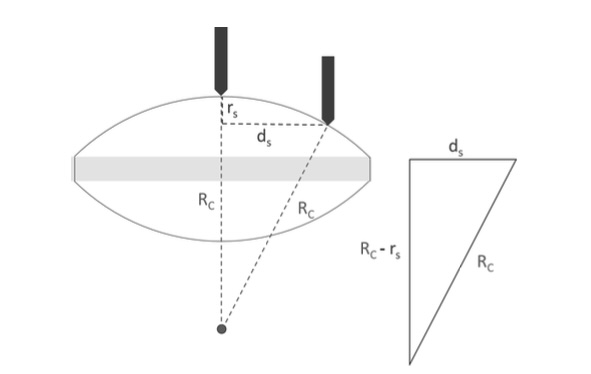
\includegraphics[width=0.5\textwidth]{Spherometer Diagram.jpeg}
    \caption{Figure 1: Spherometer Geometry (From PHYS 2007 lab manual)}
    \label{fig:spherometer}
\end{figure}

\subsection{Object at Infinity}
With object at infinity the key point was that the focal point was equal to the distance from the lens to the image. If we took equation 1 and set S=the distance from the object to the lens to infinity and after rearranging, we get:

\begin{equation}
f = S'
\end{equation}  

\subsection{The Mirror Method}
To use the mirror technique, one would arrange the apparatus like the following figure:

\begin{figure}[h]
    \centering
    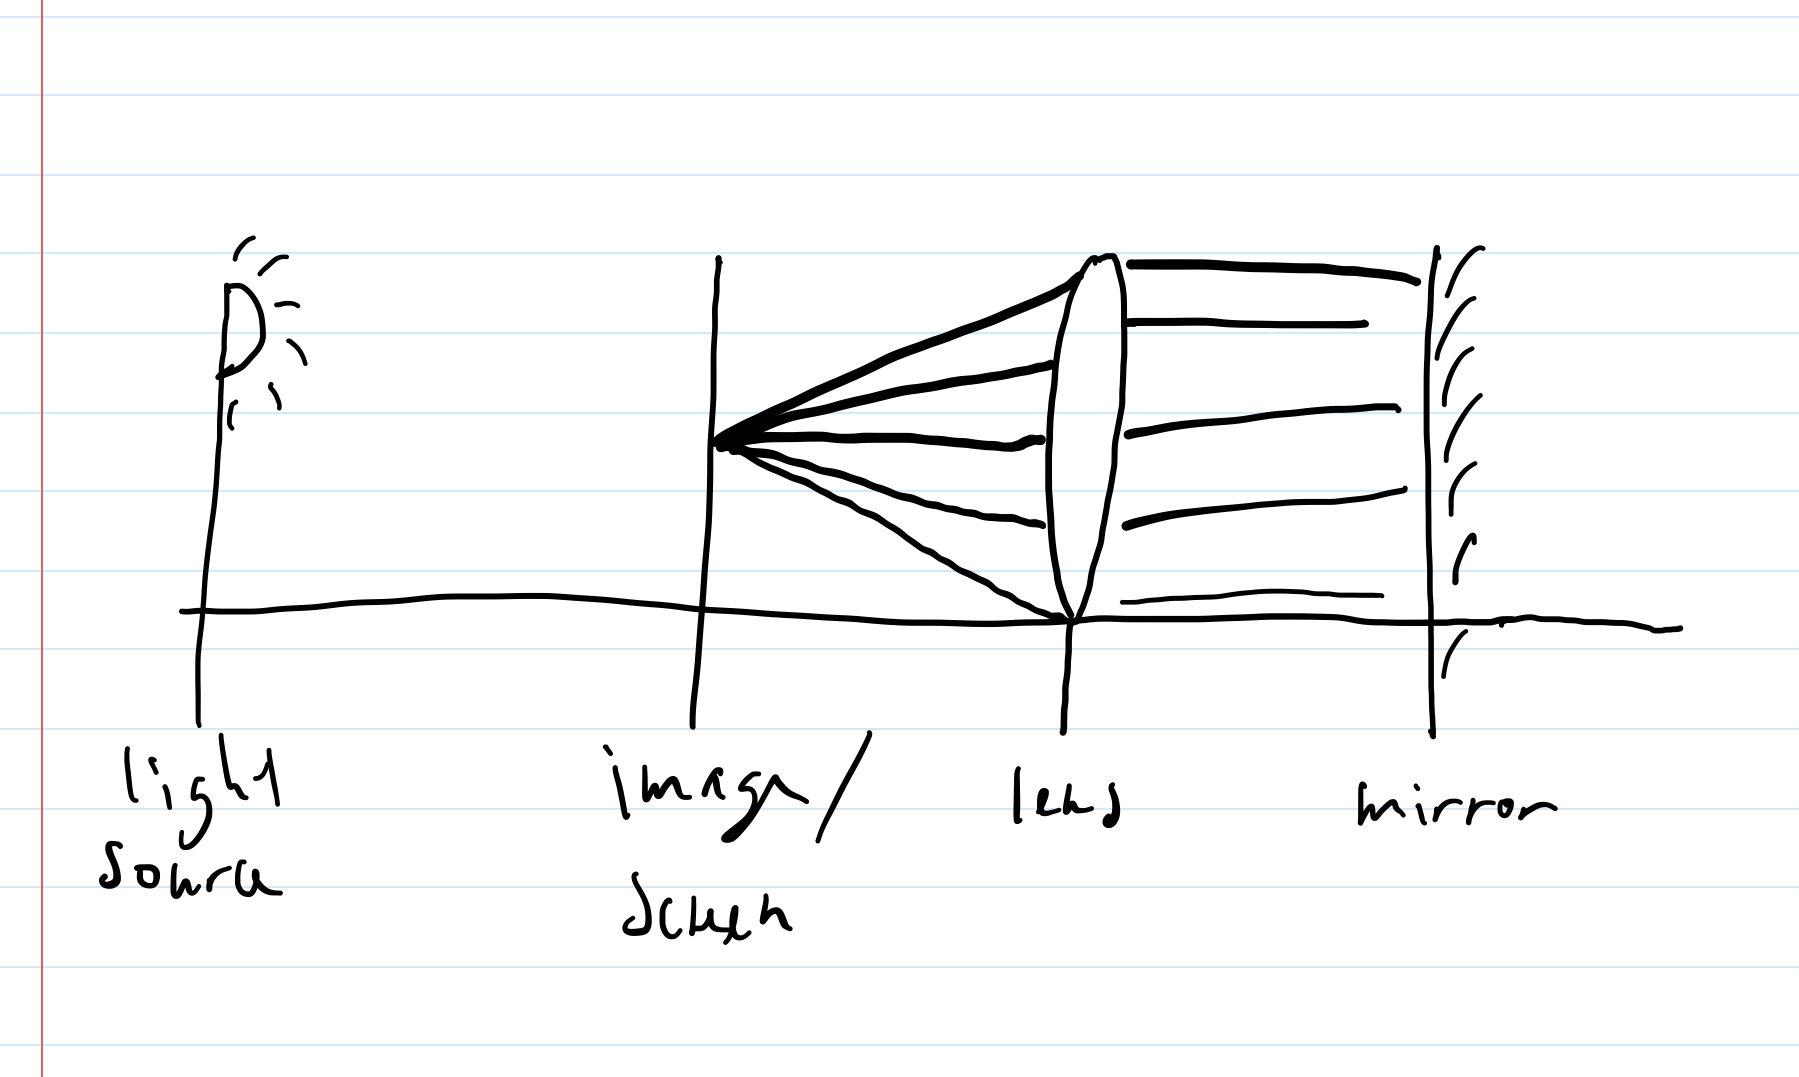
\includegraphics[width=0.5\textwidth]{The Mirror Technique.png}
    \caption{The Mirror Technique (Draw by Son Thanh Truong - Own Work)}
    \label{fig:mirror_method}
\end{figure}

In this case $f=S$, that is, the focal length is equal to the distance from the object to the lens as seen in the drawing.

\subsection{The Object at Infinity Method}
Now we’re onto the object at infinity technique. This is very similar to the mirror technique as in, the object coming at infinity hence S = Infinity. Then, following the thin lens equation (eq1) f again is equal to S’.

\subsection{The Lensmaker Equation Method}
Next let’s discuss the lens maker equation. Here is the equation:



\begin{equation}
\frac{1}{f} = (n-1) \left( \frac{1}{R_1} - \frac{1}{R_2} - \frac{(n-1)t}{n R_1 R_2} \right)
\end{equation}
Using the thin lens approximation: $t << f$ we can ignore the last term in the square brackets, and after knowing R1, R2, with the value of n which can be found out using information about the type of glass which is BK7, one can find the focal length f.

\subsection{The Magnification Technique}
To find the focal length you can also use magnification of the lens. Here is the derivation of that. M, the magnification is equal to the ratio of the size of the image to the size of the object:
\begin{equation}
M = \frac{h'}{h}
\end{equation}
From similar triangles M also equals:
\begin{equation}
M = \frac{s'}{s}
\end{equation}
There is a minus sign because the image is always flipped from the object. Combining eq1 and eq5 we get:
\begin{equation}
M = \frac{f}{f-s}
\end{equation}

After linearization:
\begin{equation}
\frac{1}{M} = -\frac{S}{f} + 1
\end{equation}

This works even with a constant offset (a) the object to lens difference:
\begin{equation}
\frac{1}{M} = -\frac{S}{f} + 1 + \frac{a}{f}
\end{equation}




\section{Experimental Setup}

\subsection{Instruments used in the experiments:}
\begin{itemize}
    \item Optics bench
    \item 1 meter ruler (range from 0 to 100cm)(Resolution 1mm)
    \item Lens holders
    \item Vertex pointers
    \item Image screen
    \item Sliding/measuring rails
    \item Mirror
    \item Spherometer(resolution 0.005mm)
    \item Venier Calipers (resolution 0.01mm)

\end{itemize}

\section{Observations:}

\subsection{Object at Infinity}
The telescope was pointed at a light source about 3 meters away. I didn’t realize that we did it wrong until after rereading my lab manual 10 mins after.
The measurements were measured using the optics bench and the ruler which has the uncertainty of 0.5 mm
\begin{table}[H]
    \centering
    \begin{tabular}{ccc}
        \hline
        Trial & $d_1$ (mm) & $d_2$ (mm) \\
        \hline
        1 & 62  & 272 \\
        2 & 569 & 775 \\
        3 & 405 & 272 \\
        4 & 237 & 508 \\
        5 & 604 & 815 \\
        \hline
    \end{tabular}
    \caption{Raw measurements for the object-at-infinity experiment. The focal length is $d_2$ minus $d_1$. Which is just the distance from the lens to the image.}
    \label{tab:object_infinity}
\end{table}

\subsection{Magnification Technique}
The Venier Caliper was used for this part and its uncertainty is 0.02 mm.
\begin{table}[H]
    \centering
    \begin{tabular}{ccc}
        \hline
        Entry & $s_o$ (mm) & $s_i$ (mm) \\
        \hline
        1 & 16.21 & 8.75 \\
        2 & 17.11 & 32.31 \\
        3 & 19.11 & 16.71 \\
        4 & 15.63 & 17.76 \\
        5 & 17.10 & 10.62 \\
        \hline
    \end{tabular}
    \caption{Raw measurements for the magnification experiment. 
    We used the Vernier Caliper to measure either the height or 
    the width, I think it was the width because the height of the
    image and of the object was very awkward to measure.
    We figured it wouldn't matter because the magnification relies
    about the size of the image not which parts to measure. 
    The magnification should be collected if we measured the same parts.
    }
    \label{tab:magnification}
\end{table}

\subsection{Thin Lens}
The ruler was used for this part and its uncertainty is 0.5 mm.

\begin{table}[H]
    \centering
    \begin{tabular}{cccc}
        \hline
        Entry & $d_1$ (cm) & $d_2$ (cm) & $d_3$ (cm) \\
        \hline
        1 & 9.5 & 48.5  & 50.3 \\
        2 & 9.5 & 55.85 & 51.5 \\
        3 & 9.5 & 58.1  & 52.2 \\
        4 & 9.5 & 60.9  & 52.5 \\
        \hline
    \end{tabular}
    \caption{Raw measurements for the thin-lens experiment. $d_1$ is the object location, $d_2$ is the lens location, and $d_3$ is the image location.}
    \label{tab:thin_lens}
\end{table}

\subsection{Mirror}
The ruler was used for this part and its uncertainty is 0.5 mm.

  \begin{table}[H]
    \centering
    \begin{tabular}{cccc}
        \hline
        Entry & $d_1$ (cm) & $d_2$ (cm) & $d_3$ \\
        \hline
        1 & 9.4 & 25.7 & 50.65 \\
        \hline
    \end{tabular}
    \caption{Raw measurements for the mirror experiment. 
    $d_1$ is the image and the screen location, 
    $d_2$ is the mirror location, and $d_3$ is the mirror location.
    I didn't realize we only had one data point if else I would've collected more.}
    \label{tab:mirror}
\end{table}  

\subsection{Lens Thickness}
The ruler was used to measure the lens thickness, and it's uncertainty is 0.5 mm.
\begin{table}[H]
    \centering
    \begin{tabular}{cccc}
        \hline
        Trial & $d_1$ (cm) & $d_2$ (cm) & $d_3$ (cm) \\
        \hline
        1 & 75.6 & 65.35 & 66.05 \\
        2 & 75.6 & 65.48 & 66.15 \\
        3 & 75.6 & 65.40 & 66.15 \\
        4 & 75.6 & 65.45 & 66.25 \\
        5 & 75.6 & 65.35 & 66.15 \\
        \hline
    \end{tabular}
    \caption{Raw lens-thickness measurements. 
    The difference between $d_2$ and $d_3$ is the lens thickness. 
    I didn't realize I only needed those two measurements.}
    \label{tab:lens_thickness}
\end{table}


\subsection{Lensmaker Equation/Spherometer}
The uncertainty for the the spherometer, $r_{s1}$ and $r_{s2}$, is 0.0025 mm. As for the Vernier caliper, $l_s$, the uncertainty is 0.02 mm.
\begin{table}[H]
    \centering
    \begin{tabular}{ccccc}
        \hline
        Entry & $r_{s1}$ (mm) & $r_{s2}$ (mm) & $l_s$ (mm) & Calibration (mm) \\
        \hline
        1 & 1.16 & 1.15 & 22.58 & -0.13 \\
        2 & 1.16 & 1.16 & 21.57 & -0.13 \\
        3 & 1.16 & 1.16 & 22.07 & -0.13 \\
        4 & 1.16 & 1.16 & --    & -0.13 \\
        5 & 1.16 & 1.16 & --    & -0.13 \\
        \hline
    \end{tabular}
    \caption{Raw spherometer measurements. $r_{s1}$ and $r_{s2}$ are the radii measured by the spherometer for two sides of the lens, 
    $l_s$ is the length measured by the Vernier caliper, 
    and Calibration is the Spherometer calibration correction applied to all Spherometer reading.}
    \label{tab:spherometer}
\end{table}

\section{Data Analysis}
Please refer to the python analysis PDF attachment.

\section{Discussion}
I felt that my partner was very rushed, he didn't 
want to talk to me, and we got terrible measurements 
because he rushed us and he was quite agressive and 
I couldn't question his authority because I wanted 
to keep the peace. If things don't go well with my
next lab partner, I think I'll ask the prof to have
me do the lab alone. It was so rushed and the measurements 
were so low quality. We even forgot to take the S measurements
for the magnification technique. If things went better it would 
have been a lot more fun and that would make the learning so much easier.

The results were very mediocre and it was a nightmare working with that guy.
It was not on par with what an exceptional well done lab would be like.
Some sections when the data was analyzed were well done, but on other sections
there were missing measurements or we only did one trial.

All in all, I did get to experience different ways to focus on one thing 
which was the focal length of the lens. So I would say that the goal of
these experiment was achieved. I re-remembered the errors for the two 
different instruments, digital and analog.
I was able to practice error propagation few times throughout the experimental write up. 
Next time I think that I will get a better mark and have better performance
inside the laboratory after having a lot more experience gathered to boost my grades.



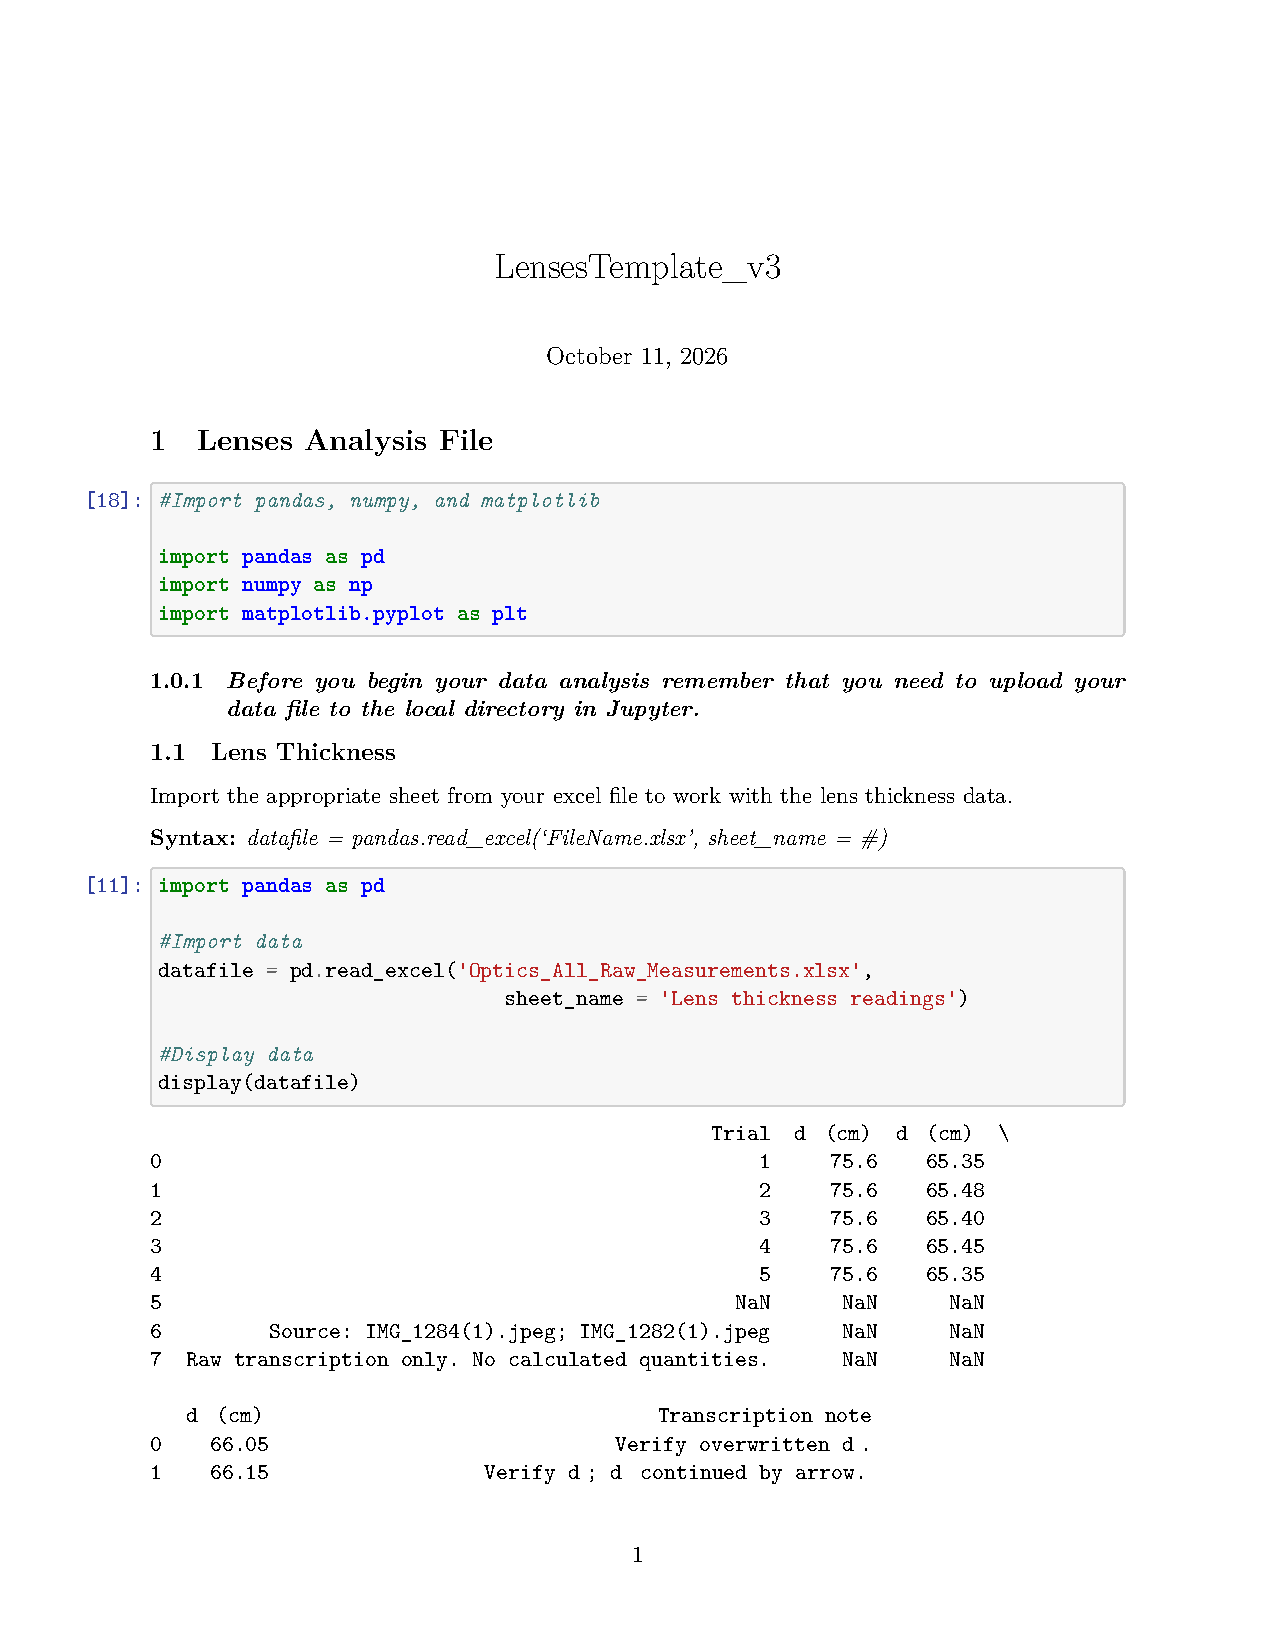
\includepdf[pages=-]{LensesTemplate_v3.pdf}
\end{document}